\documentclass [../article.tex]{subfiles}
\begin{document}
  \section{Image Processing}
  The Fourier Transform converts a domain into a frequency domain.
  As we saw earlier, the Fourier Transform in audio signals takes
  a continuous time domain and converts it into a frequency domain.
  In image processing, the Fourier Transform converts a spatial
  domain into a frequency domain (Smith 24).  The Fourier Transform
  in image processing allows us to access the geometric
  characteristics of an image (Fisher 3).  By having access to the
  geometric characteristic, we are able to modify the image by
  changing some of those characteristics.

  In order to modify the characteristics of an image, we apply
  filters. Most of the time we apply filters to the original
  image. However, this is not always the most efficient way to
  manipulate an image. When we want to smooth, sharpen, and enhance
  an image, it is easier to take the Discrete Fourier Transform,
  apply the filters, and then take the inverse Discrete Fourier
  Transform to obtain the image with the changes (Ludwig 3).  It
  is easier to apply the filter in the Discrete Fourier Transform
  because sharpening, enhancing, and smoothing an image are all
  consequences of convolution.  The Discrete Fourier Transform
  allows convolution to occur easier mathematically since
  convolution in the spatial domain becomes simply multiplication
  in the frequency domain (Smith 24).  Therefore, applying filters
  in the frequency domain is much easier than applying filters in
  the spatial domain.

  Because images are in two dimension, we cannot calculate the
  Fourier Transform using a one dimension formula, like we did in
  audio signals.  Therefore, we need to manipulate the Fourier
  Transform formula to take care of this extra dimension.

  The one dimensional (1D) Discrete Fourier Transform formula is:
  \[ F(k) = \sum_{x=0}^{N-1}f(x)e^{-i2\pi kx/N} \]
  We take the DFT of the rows, $F(k)$, and then the DFT of the
  columns, $F(l)$:
  \[F(k) = \sum_{x=0}^{N-1}f(x)e^{-i2\pi kx/N}
    \phantom{space}
    F(l) = \sum_{y=0}^{N-1}f(y)e^{-i2\pi ly/N}\]
  Then we multiply them together:
  \begin{align*}
    F(k)F(l) = F(k,l) &=
    \sum_{x=0}^{N-1}f(x)e^{-i2\pi kx/N}
    \sum_{y=0}^{N-1}f(y)e^{-i2\pi ly/N}\\
    {} &= \sum_{x=0}^{N-1}\sum_{y=0}^{N-1}f(x,y)
    e^{-i2\pi kx/N}e^{-i2\pi ly/N}\\
    {} &= \sum_{x=0}^{N-1}\sum_{y=0}^{N-1}f(x,y)
    e^{-i2\pi kx/N - i2\pi ly/N}\\
    {} &= \sum_{x=0}^{N-1}\sum_{y=0}^{N-1}f(x,y)
    e^{-i(kx+ly)2\pi/N }
  \end{align*}

  Therefore, we get the 2 dimensional (2D) Discrete Fourier
  Transform formula:
  \[\sum_{x=0}^{N-1}\sum_{y=0}^{N-1}f(x,y)e^{-i(kx+ly)2\pi/N}\]
  where $f(x,y)$ is the image of the spatial domain.

  Note that this formula only works for an $N \times N$ image,
  where $N$ is a power of 2. If the image is not $N \times N$,
  add the necessary 0 vectors in either the rows or columns
  until it is.

  Similarly, we can derive the 2D inverse DFT formula from the
  1D inverse DFT formula:
  \[f(x,y) = \frac{1}{N^2}\sum_{k=0}^{N-1}\sum_{l=0}^{N-1}
    F(k,l)e^{i2\pi(kx/N+ly/N)}\]
  Note the presence of $1/N^2$. This is sometimes present
  in the Discrete Fourier Transform formula. However,
  $1/N^2$ should not be present in both the DFT and the
  inverse DFT.

  The Discrete Fourier Transform is complex, therefore, having
  real and imaginary parts.  In image processing, instead of
  displaying the DFT as real and imaginary images, we display
  the DFT using magnitude and phase.

  The magnitude can be calculated by:
  \[\text{Mag}(F) = \sqrt{\text{Real}(F)^2 + \text{Imaginary}(F)^2}\]

  The phase can be calculated by:
  \[\text{Phase}(F) = \arctan\left(
  \frac{\text{Imaginary(F)}}{\text{Real(F)}}\right)\]

  The magnitude tells us how much a certain frequency is present,
  while the phase tells us where the frequency is in the image
  (Brayer 2).  Even though the phase typically holds more
  information, we only display the magnitude image of the DFT.
  When applying filters, we do not want to change where the
  frequency is located, but manipulate the presence of the
  frequency themselves.  Therefore, the information pertinent
  to us is the magnitude.

  Let's look at an example.
  \begin{figure}[htbp]
  \minipage{0.32\textwidth}
    \includegraphics[width=\linewidth]{jocelyn/01/original.png}
    \caption{The Original Image}
    \label{fig:original1}
  \endminipage\hfill
  \minipage{0.32\textwidth}
    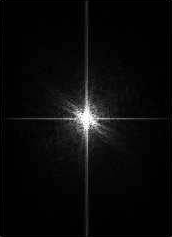
\includegraphics[width=\linewidth]{jocelyn/01/mag.png}
    \caption{Magnitude of our Transform}
    \label{fig:mag1}
  \endminipage\hfill
  \minipage{0.32\textwidth}%
    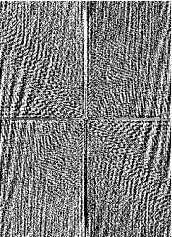
\includegraphics[width=\linewidth]{jocelyn/01/phase.png}
    \caption{Phase of our Transform}
    \label{fig:phase1}
  \endminipage
  \end{figure}
  Figure~\ref{fig:original1} is our original image. While
  figures~\ref{fig:mag1} and \ref{fig:phase1} show the
  magnitude and phase of the Fourier Transform respectively.

  Even though the information pertinent to us is the magnitude,
  we do not want to just ignore the phase. We want to preserve
  the phase because that contains important information of where
  each frequency is located. Without the phase, our image will be
  corrupted.  In our example, if we only reconstructed the image
  using the magnitude, we would end up with figure~\ref{fig:magonly}.
  Therefore, even though the magnitude contains the most
  information, we still must protect and preserve the phase
  in order to obtain our image. Taking the inverse Discrete Fourier
  Transform of the phase without the magnitude, we will get an
  outline of what the image is without any other color detail
  (Kundur 17-19). In our example, we would get the image in
  figure~\ref{fig:phaseonly} Note that because we
  preserved the phase, we know where each frequency should be
  located, therefore we will get an outline of the image.
  \begin{figure}[htbp]
  \minipage{0.32\textwidth}
    \includegraphics[width=\linewidth]{jocelyn/01/original.png}
    \caption{The Original Image}
    \label{fig:original1_}
  \endminipage\hfill
  \minipage{0.32\textwidth}
    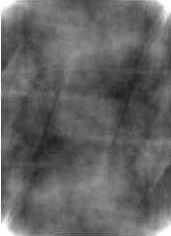
\includegraphics[width=\linewidth]{jocelyn/01/magonly.png}
    \caption{Inverse of Magnitude Only}
    \label{fig:magonly}
  \endminipage\hfill
  \minipage{0.32\textwidth}%
    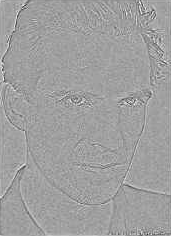
\includegraphics[width=\linewidth]{jocelyn/01/phaseonly.png}
    \caption{Inverse of Phase Only}
    \label{fig:phaseonly}
  \endminipage
  \end{figure}

  The results of the Discrete Fourier Transform show an image
  that contains components of all frequencies.  The higher the
  frequency is, the lower the frequency magnitude is.  Therefore,
  low frequencies contain more information about the image than
  the higher frequencies.  In order to obtain and keep the most
  information that we can, we take the logarithmic of the
  magnitude.that we can, we take the logarithmic of the magnitude.
  es while compressing high frequencies.  However, note that if
  an image contains important information in the higher
  frequencies, applying the logarithmic operator may lead
  to information loss (Fisher 3).

  In most Discrete Fourier Transform images, the Fourier image is
  shifted such that $F(0,0)$, the image mean, is centered in the
  middle (Fisher 3).  Hence, the further from the origin, the
  higher the frequency, the lower the magnitude.  In all of the
  pictures of the Discrete Fourier Transform in image processing in
  this paper, we will shift the Fourier image such that the image
  mean is centered in the middle.  All Discrete Fourier Transform
  images will also represent the logarithmic of the magnitude of the
  Fourier Transform in 2D as well.

  The purpose of using Fourier Transform in image processing is to
  apply filters in order to change the original image.  I will give
  a few examples of manipulating the Fourier Transform and  showing
  what the results would be like if we were to take the inverse
  Fourier Transform back to the original image.
  \begin{figure}[htbp]
    \minipage{0.4\textwidth}
      \includegraphics[width=\linewidth]{jocelyn/02/original.png}
      \caption{Original}
      \label{fig:original2}
    \endminipage\hfill
    \minipage{0.4\textwidth}
      \includegraphics[width=\linewidth]{jocelyn/02/originalspectrum.png}
      \caption{Spectrum}
      \label{fig:spectrum2}
    \endminipage
  \end{figure}

  When we only take the lower frequencies and zero out the higher
  frequencies in the Fourier Transform image, we obtain the spectrum
  in figure~\ref{fig:lpspectrum} who's inverse fourier transform
  is shown in figure~\ref{fig:lpinverse}.
  \begin{figure}[htbp]
    \minipage{0.4\textwidth}
      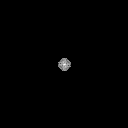
\includegraphics[width=\linewidth]{jocelyn/02/lpspectrum.png}
      \caption{Low Pass Spectrum}
      \label{fig:lpspectrum}
    \endminipage\hfill
    \minipage{0.4\textwidth}
      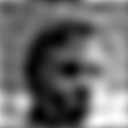
\includegraphics[width=\linewidth]{jocelyn/02/lpinverse.png}
      \caption{Low Pass Inverse}
      \label{fig:lpinverse}
    \endminipage
  \end{figure}
  Notice here in the Fourier Transform image we have the brightest
  spot preserved.  However, we did lose quite a bit of high
  frequency and even some of the lower frequencies.  Many of the
  bright spots in the original Fourier Transform image is lost.
  This is why the image after taking the inverse Fourier Transform
  of the new Fourier Transform image is so blurry.  We lost too much
  information in the Fourier Transform.

  Earlier in this section we said that the magnitude of the Fourier
  Transform told us how much of a frequency component was present in
  the image.  This becomes apparent when we keep the high
  frequencies but zero out the lower frequencies in the Fourier
  Transform. This effect is highlighted in figure~\ref{fig:hpinverse}
  which was obtained via the inverse of the spectrum shown in
  figure~\ref{fig:hpspectrum}.
  \begin{figure}[htbp]
    \minipage{0.4\textwidth}
      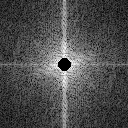
\includegraphics[width=\linewidth]{jocelyn/02/hpspectrum.png}
      \caption{High Pass Spectrum}
      \label{fig:hpspectrum}
    \endminipage\hfill
    \minipage{0.4\textwidth}
      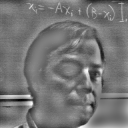
\includegraphics[width=\linewidth]{jocelyn/02/hpinverse.png}
      \caption{High Pass Inverse}
      \label{fig:hpinverse}
    \endminipage
  \end{figure}

  Since the lower frequencies contain more information, the color of
  the image is mostly lost.  However, because we preserved the phase
  and still have the higher frequencies, we are able to obtain an
  outline of an image.  This is known as edge detection as the
  Fourier Transform is able to show the highly contrasted color
  changes of the original image.

  The following images take out frequencies above and below a
  certain band limit.  So within this band in the Fourier
  Transform shown in figure~\ref{fig:bp1spectrum}, it becomes
  figure~\ref{fig:bp1inverse} after an inverse fourier transform.
  \begin{figure}[htbp]
    \minipage{0.4\textwidth}
      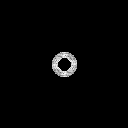
\includegraphics[width=\linewidth]{jocelyn/02/bp1spectrum.png}
      \caption{Band Pass Spectrum}
      \label{fig:bp1spectrum}
    \endminipage\hfill
    \minipage{0.4\textwidth}
      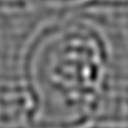
\includegraphics[width=\linewidth]{jocelyn/02/bp1inverse.png}
      \caption{Band Pass Inverse}
      \label{fig:bp1inverse}
    \endminipage
  \end{figure}

  In the following image, we did the same thing.  However, this time
  we decreased the size of the band in the Fourier Transform.  Note
  that because the band is smaller, we have less information about
  the image.  Therefore, the inverse Fourier Transform image in
  figure~\ref{fig:bp2inverse}
  is much blurrier than the inverse Fourier Transform of the image
  in figure~\ref{fig:bp1inverse}
  \begin{figure}[htbp]
    \minipage{0.4\textwidth}
      
\includegraphics[width=\linewidth]{jocelyn/02/bp2spectrum.png}
      \caption{Band Pass Spectrum}
      \label{fig:bp2spectrum}
    \endminipage\hfill
    \minipage{0.4\textwidth}
      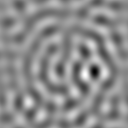
\includegraphics[width=\linewidth]{jocelyn/02/bp2inverse.png}
      \caption{Band Pass Inverse}
      \label{fig:bp2inverse}
    \endminipage
  \end{figure}

  Finally we take a wide high frequency band limit in
  figure~\ref{fig:bp3spectrum} and then reduce it's width
  in figure~\ref{fig:bp4spectrum}.
  \begin{figure}[htbp]
    \minipage{0.4\textwidth}
      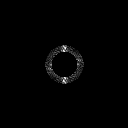
\includegraphics[width=\linewidth]{jocelyn/02/bp3spectrum.png}
      \caption{Band Pass Spectrum}
      \label{fig:bp3spectrum}
    \endminipage\hfill
    \minipage{0.4\textwidth}
      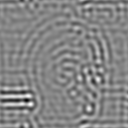
\includegraphics[width=\linewidth]{jocelyn/02/bp3inverse.png}
      \caption{Band Pass Inverse}
      \label{fig:bp3inverse}
    \endminipage
  \end{figure}
  \begin{figure}[htbp]
    \minipage{0.4\textwidth}
      
\includegraphics[width=\linewidth]{jocelyn/02/bp4spectrum.png}
      \caption{Band Pass Spectrum}
      \label{fig:bp4spectrum}
    \endminipage\hfill
    \minipage{0.4\textwidth}
      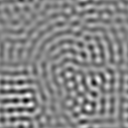
\includegraphics[width=\linewidth]{jocelyn/02/bp4inverse.png}
      \caption{Band Pass Inverse}
      \label{fig:bp4inverse}
    \endminipage
  \end{figure}

  Note that the smaller band of higher frequency looks more similar
  to the larger band of higher frequency than the smaller band of
  lower frequency and the larger band of lower frequencies.  This is
  again because lower frequencies contain more information.
  Therefore, the change of the band in the lower frequencies is more
  significant than changing the band in the higher frequencies.

  Also note that even though we lost a lot of information in the
  images after manipulating the original pictures Fourier Transform,
  we can still see a rough outline of what the image looks like.
  This is a result of preserving the phase.

  Although it is nice to know how the changes in the Fourier
  Transform affects the images, typically in image processing, we
  won’t be omitting many important frequencies, but enhancing and
  sharpening them.

  In the next example, I will be using figure~\ref{fig:sharporig}
  as the original photo while figure~\ref{fig:sharporigspectrum}
  is it's spectrum.
  \begin{figure}[htbp]
    \minipage{0.4\textwidth}
      \includegraphics[width=\linewidth]{jocelyn/03/sharp/original.png}
      \caption{Original Image}
      \label{fig:sharporig}
    \endminipage\hfill
    \minipage{0.4\textwidth}
      \includegraphics[width=\linewidth]{jocelyn/03/sharp/originalspectrum.png}
      \caption{Original Spectrum}
      \label{fig:sharporigspectrum}
    \endminipage
  \end{figure}
  Then we apply our filters to these images to obtain the sharpened
  image in figure~\ref{fig:sharpfiltered} with it's corresponding
  spectrum in figure~\ref{fig:sharpfilteredspectrum}
  \begin{figure}[htbp]
    \minipage{0.4\textwidth}
      \includegraphics[width=\linewidth]{jocelyn/03/sharp/filtered.png}
      \caption{Filtered Image}
      \label{fig:sharpfiltered}
    \endminipage\hfill
    \minipage{0.4\textwidth}
      \includegraphics[width=\linewidth]{jocelyn/03/sharp/filteredspectrum.png}
      \caption{Filtered Spectrum}
      \label{fig:sharpfilteredspectrum}
    \endminipage
  \end{figure}
  Notice that the frequencies of the higher magnitude frequencies
  are lighter than the original high frequencies in the original
  Fourier Transform image.  In order to obtain this, we kept the
  lower frequencies the same, but every frequency above 96, we
  multiplied by the Fourier Transform coefficients by 4.

  The Fourier Transform is also used to reduce noise.
  \begin{figure}[htbp]
  \minipage{0.32\textwidth}
    \includegraphics[width=\linewidth]{jocelyn/03/noise/original.png}
    \caption{Original Image}
    \label{fig:orignoise}
  \endminipage\hfill
  \minipage{0.32\textwidth}
    \includegraphics[width=\linewidth]{jocelyn/03/noise/originalspectrum.png}
    \caption{Original Spectrum}
    \label{fig:orignoisespectrum}
  \endminipage\hfill
  \minipage{0.32\textwidth}%
    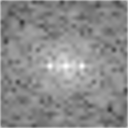
\includegraphics[width=\linewidth]{jocelyn/03/noise/originalspectrumzoom.png}
    \caption{Zoomed Spectrum}
    \label{fig:origzoomed}
  \endminipage
  \end{figure}
  In figure~\ref{fig:orignoise}, we have a picture of goofy. He
  has a cosine function embedded in him, which is why we have the
  ``noise'' or the rolls in the image. The cosine function can
  be seen in the Fourier Transform image
  (figure~\ref{fig:orignoisespectrum}).  The center of
  the Fourier Transform image has three bright dots.  In order to
  see the cosine function more clearly in the Fourier Transform, we
  zoomed in on the center of the Fourier Transform (figure~\ref{fig:origzoomed}).  The outer dots represent the cosine function.
  Therefore, in order to remove the noise, we must take out the
  cosine function.  So, we zero out the dots in the Fourier
  Transform.  When we do that, we get figures~\ref{fig:filterednoise}-\ref{fig:filteredzoom}
  \begin{figure}[htbp]
  \minipage{0.32\textwidth}
    \includegraphics[width=\linewidth]{jocelyn/03/noise/filtered.png}
    \caption{Filtered Image}
    \label{fig:filterednoise}
  \endminipage\hfill
  \minipage{0.32\textwidth}
    \includegraphics[width=\linewidth]{jocelyn/03/noise/filteredspectrum.png}
    \caption{Filtered Spectrum}
    \label{fig:filteredspectrum}
  \endminipage\hfill
  \minipage{0.32\textwidth}%
    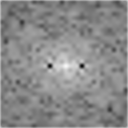
\includegraphics[width=\linewidth]{jocelyn/03/noise/filteredspectrumzoom.png}
    \caption{Zoomed Spectrum}
    \label{fig:filteredzoom}
  \endminipage
  \end{figure}
  Notice that the outer bright dots are removed from the Fourier
  Transform.  Therefore, the original image is smoother than before.

  The Fourier Transform in image processing allows us to change some
  characteristics of an image in the spatial domain.  By taking the
  Fourier Transform of every row of an N x N image and taking the
  Fourier Transform of every column, we are able to obtain a formula
  to calculate the Fourier Transform of a 2D image.  By taking the
  magnitude, we can display the Fourier Transform image.  In order
  to change the characteristics of an image in the spatial domain,
  we use the multiplication operator in the frequency domain.
  Sometimes we multiply the Fourier coefficients by zero in certain
  frequencies in order to remove those frequencies.  By doing so, we
  can smooth out an image.  By strategically multiplying certain
  Fourier coefficients in the frequency domain, we are able to
  enhance images.  However, we cannot just focus on the magnitude of
  the Fourier Transform.  We must preserve the phase as well.
  Preserving the phase of every image is important as the phase
  tells us where each frequency is located.
\end{document}
